% Document class
\documentclass[a4paper,11pt,twoside]{book}

% ------------------------------------------------------------------------------
% Encoding, Language, Typography
% ------------------------------------------------------------------------------
\usepackage[utf8]{inputenc}
\usepackage[T1]{fontenc}
\usepackage[ngerman,english]{babel}
\usepackage{microtype}
\usepackage{subfiles}
\microtypecontext{spacing=nonfrench}
\SetTracking{encoding={*}, shape=sc}{40}
\usepackage{indentfirst}
\usepackage{textcomp}

% ------------------------------------------------------------------------------
% Page Geometry and Layout
% ------------------------------------------------------------------------------
\usepackage[margin=1.1in]{geometry}
\usepackage{fancyhdr}
\usepackage{mparhack}
\usepackage{booktabs}
\usepackage{titlesec}
\usepackage[Lenny]{fncychap}
\ChTitleAsIs

% Widows and orphans
\clubpenalty = 10000
\widowpenalty = 10000
\displaywidowpenalty = 10000

% ------------------------------------------------------------------------------
% Fonts and Symbols
% ------------------------------------------------------------------------------
\usepackage{amsmath, amssymb, amstext, amsfonts, mathtools}
\usepackage{mathpazo} % Palatino with matching math
% \usepackage{eulervm} % Optional math font
\usepackage[b]{esvect}  % Vector notation
\usepackage{siunitx}    % Scientific units
\sisetup{
    uncertainty-mode = separate
}
\DeclareSIUnit\yr{yr}
\DeclareSIUnit\sr{sr}


% ------------------------------------------------------------------------------
% Graphics and Figures
% ------------------------------------------------------------------------------
\usepackage{graphicx}
\usepackage{subcaption}
\usepackage{wrapfig}
\usepackage[export]{adjustbox}
\usepackage{tikz}
\usepackage{rotating}
%\usepackage{subfig}
\usepackage[rightcaption]{sidecap}
\sidecaptionvpos{figure}{t}
\usepackage[labelfont=bf,font=small,margin=10pt,format=plain,tableposition=top]{caption}
\graphicspath{{figures/}}

% ------------------------------------------------------------------------------
% Listings and Code
% ------------------------------------------------------------------------------
\usepackage{listings}
\lstset{
    frame=single,
    breaklines=true,
    postbreak=\raisebox{0ex}[0ex][0ex]{\ensuremath{\color{red}\hookrightarrow\space}},
    basicstyle=\ttfamily,
    columns=fullflexible,
    showstringspaces=false,
    commentstyle=\color{gray}\upshape
}

\lstdefinelanguage{numpy}{
    keywords={and, del, from, not, while, as, elif, global, or, with,
              assert, else, if, pass, yield, break, except, import, print,
              class, exec, in, raise, continue, finally, is, return, def, for, lambda, try},
    morekeywords={numpy, fft, mean}
}

\lstdefinelanguage{XML}{
    basicstyle=\ttfamily\color{darkblue}\bfseries\footnotesize,
    morestring=[b]",
    morestring=[s]{>}{<},
    morecomment=[s]{<?}{?>},
    stringstyle=\color{black},
    identifierstyle=\color{darkblue},
    keywordstyle=\color{cyan},
    morekeywords={xmlns, version, type},
    breaklines=true
}

% ------------------------------------------------------------------------------
% Colors
% ------------------------------------------------------------------------------
\usepackage{xcolor}
\usepackage{colortbl}
\definecolor{darkred}{rgb}{0.5,0,0}
\definecolor{firebrick}{rgb}{0.75,0.125,0.125}
\definecolor{darkgreen}{rgb}{0,0.5,0}
\definecolor{lightgray}{gray}{0.9}
\definecolor{gray}{rgb}{0.4,0.4,0.4}
\definecolor{darkblue}{rgb}{0.0,0.0,0.6}
\definecolor{cyan}{rgb}{0.0,0.6,0.6}

% ------------------------------------------------------------------------------
% Utility and Misc Packages
% ------------------------------------------------------------------------------
\usepackage{etoolbox}
\usepackage{xparse}
\usepackage{xspace}
\usepackage{duckuments}  % Presumably for testing images
\usepackage{changes}      % Track changes
\usepackage{todonotes}    % TODO comments
\usepackage{epigraph}
\setlength{\epigraphwidth}{1.0\textwidth}
\usepackage{python}       % For embedding Python code (if applicable)
\usepackage{lipsum}
\usepackage{blindtext}
\usepackage{TitleEnglish}
\usepackage{TitleSpanish}
\usepackage{TitleGerman}
\usepackage{tabularx}

\input utilities
\input values

% ------------------------------------------------------------------------------
% Title, Author, Metadata
% ------------------------------------------------------------------------------
\newcommand{\thetitle}{Measurement of the Second Knee in the Cosmic Ray Spectrum with the Surface Detector of the Pierre Auger Observatory}
\title{\thetitle}
\author{Gabriel Brichetto Orquera}
\date{}

% ------------------------------------------------------------------------------
% Bibliography
% ------------------------------------------------------------------------------
\usepackage[
    backend=biber,
    style=phys,
    citestyle=numeric-comp,
    biblabel=brackets,
    sorting=none,
    giveninits=true,
    maxbibnames=6,
    minbibnames=1
]{biblatex}
\addbibresource{bibiblioteca.bib}
\DeclareFieldFormat[article,inproceedings,thesis]{title}{\mkbibemph{#1}}

% ------------------------------------------------------------------------------
% Hyperlinks and References
% ------------------------------------------------------------------------------
\usepackage{hyperref}
\hypersetup{
  pdfsubject={Ph.D. thesis},
  pdftitle={\thetitle},
  pdfauthor={P. Gabriel Brichetto Orquera},
  pdfcreator={LaTeX, pdfTeX},
  pdfkeywords={astroparticle physics, ultra-high energy cosmic rays, Pierre Auger Observatory, energy spectrum, unfolding},
  colorlinks=true,
  plainpages=false,
  linkcolor=black,
  citecolor=black,
  urlcolor=blue,
  bookmarksopen=false,
  linktocpage=true
}

\usepackage[capitalize]{cleveref}

% ------------------------------------------------------------------------------
% Glossaries & Acronyms
% ------------------------------------------------------------------------------
\usepackage[acronym]{glossaries}
\input acronyms
\makeglossaries

% ------------------------------------------------------------------------------
% Floating and TOC control
% ------------------------------------------------------------------------------
\setcounter{topnumber}{4}
\renewcommand{\topfraction}{1.}
\setcounter{bottomnumber}{0}
\renewcommand{\bottomfraction}{0}
\setcounter{totalnumber}{4}
\renewcommand{\textfraction}{0.}
\renewcommand{\floatpagefraction}{1.}
\setcounter{tocdepth}{1}
\setcounter{secnumdepth}{3}

% ------------------------------------------------------------------------------
% Hyphenation rules (add as needed)
% ------------------------------------------------------------------------------
\hyphenation{
  % Example: Pro-to-koll-in-stan-zen
}

% ------------------------------------------------------------------------------
% Math and Bold Handling in Section Titles
% ------------------------------------------------------------------------------
\makeatletter
\DeclareRobustCommand*{\bfseries}{%
  \not@math@alphabet\bfseries\mathbf
  \fontseries\bfdefault\selectfont
  \boldmath
}
\makeatother

\begin{document}

\frontmatter

\sisetup{per-mode = symbol,
         detect-all,
         tight-spacing = true,
         separate-uncertainty = true} % if false it will give uncertainty 1.2 +- 0.3 as 1.2(3)

% tex file following format specified by the doctoral committee
% fill in with your details
\input title

% abstracts
\input abstract_english
\input abstract_spanish
\input abstract_german

\chapter*{Acknowledgments}
\input thanks

\input dedicatoria

\selectlanguage{english}

\let\oldbaselinestretch=\baselinestretch%
\renewcommand{\baselinestretch}{1.15}%
\large\normalsize%

\renewcommand{\baselinestretch}{\oldbaselinestretch}%
\large\normalsize%


\microtypesetup{protrusion=false}
\tableofcontents
\microtypesetup{protrusion=true}

\clearpage

\mainmatter


\subfile{Chapter_1_Introduction}

\subfile{Chapter_2_Cosmic_rays}

\subfile{Chapter_3_Auger}

\subfile{Chapter_4_SD433_dataset}

\subfile{Chapter_5_Energy_reconstruction}

\subfile{Chapter_6_SD433_spectrum}

\subfile{Chapter_7_Combined_spectrum}

\subfile{Chapter_8_Comparison}

\subfile{Chapter_9_Summary}

% \chapter{The SD-750}
% \label{chapter:SD-750}
% \input chapter_8_SD-750

% \chapter{Combined SD Spectrum}
% \label{chapter:Combined_Spectrum}
% \input chapter_9_Winds_of_winter

% \chapter{Summary and outlook}
% \label{chapter:summary}
% \input chapter_10_A_Dream_of_Spring

\printbibliography

% Acronyms
\cleardoublepage
\phantomsection
\addcontentsline{toc}{chapter}{Acronyms}
\printglossary[type=\acronymtype, title=Acronyms,toctitle=Acronyms]

% List of Tables
\phantomsection % To correctly anchor hyperlinks
\addcontentsline{toc}{chapter}{\listtablename} % Add "List of Tables" to TOC
\listoftables

% List of Figures
\phantomsection % To correctly anchor hyperlinks
\addcontentsline{toc}{chapter}{\listfigurename} % Add "List of Figures" to TOC
\listoffigures

\begin{appendix}
\chapter{Supplementary material for \cref{chapter:SD433_Spectrum}}
\label{app:chap_spectrum}

\chapter{Supplementary material for \cref{chapter:sd750_combined_spectrum}}
\label{appendix:chapter_combined}

\begin{figure}[htbp]
    \centering
    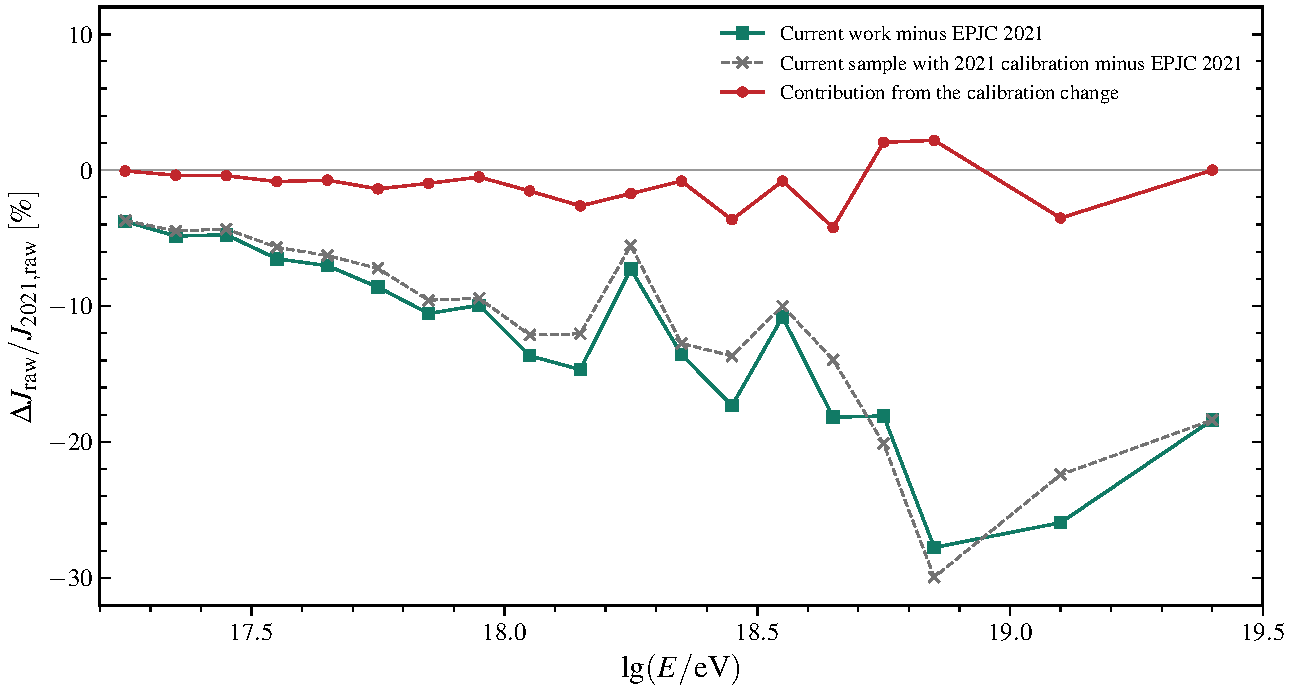
\includegraphics[width=\linewidth]{figures/chapter_combined/sd750_flux_difference_calibration.pdf}
    \caption{Relative difference between the updated raw \sd{750} spectrum and the spectrum published in 2021~\cite{PierreAuger:2021:InfillSpectrum} (green squares).
    The gray crosses show the difference obtained when the current event sample is assigned energies using the 2021 calibration relation, keeping its selection, exposure and energy bins unchanged.
    The red circles show the contribution from the calibration change, calculated as the difference between the two versions of the current spectrum.
    All differences are divided by the published raw flux, so the green values are the sum of the gray and red values.
    The calibration relations are evaluated at their nominal parameter values.
    Statistical uncertainties are not shown.}
    \label{fig:sd750_flux_difference_calibration}
\end{figure}

\end{appendix}

%\input erklaerung

\end{document}
